\chapter{Engineering System Schematics}
\label{chap:engineering-schematics}

This chapter adds the high-level engineering interconnect sheets for the current RUDRAv4 hardware stack.  The intent is to provide a clean, reviewable system schematic that sits one level above the pictorial wiring image: it separates compute power, motor power, USB/data connections, packetized Sabertooth control, encoder feedback, and IMU wiring into two readable sheets.

\begin{designbox}{How to use these sheets}
Use these schematics as the engineering map for bring-up and troubleshooting.  Use Sheet 1 for power-domain and NUC-level wiring checks.  Use Sheet 2 for Teensy, Sabertooth, encoder, IMU, and PS2 controller pin-level checks.  The schematics intentionally avoid pictorial wire clutter and use named nets/off-page references so the drawing remains readable in print.
\end{designbox}

\begin{landscape}
\begin{figure}[p]
\centering
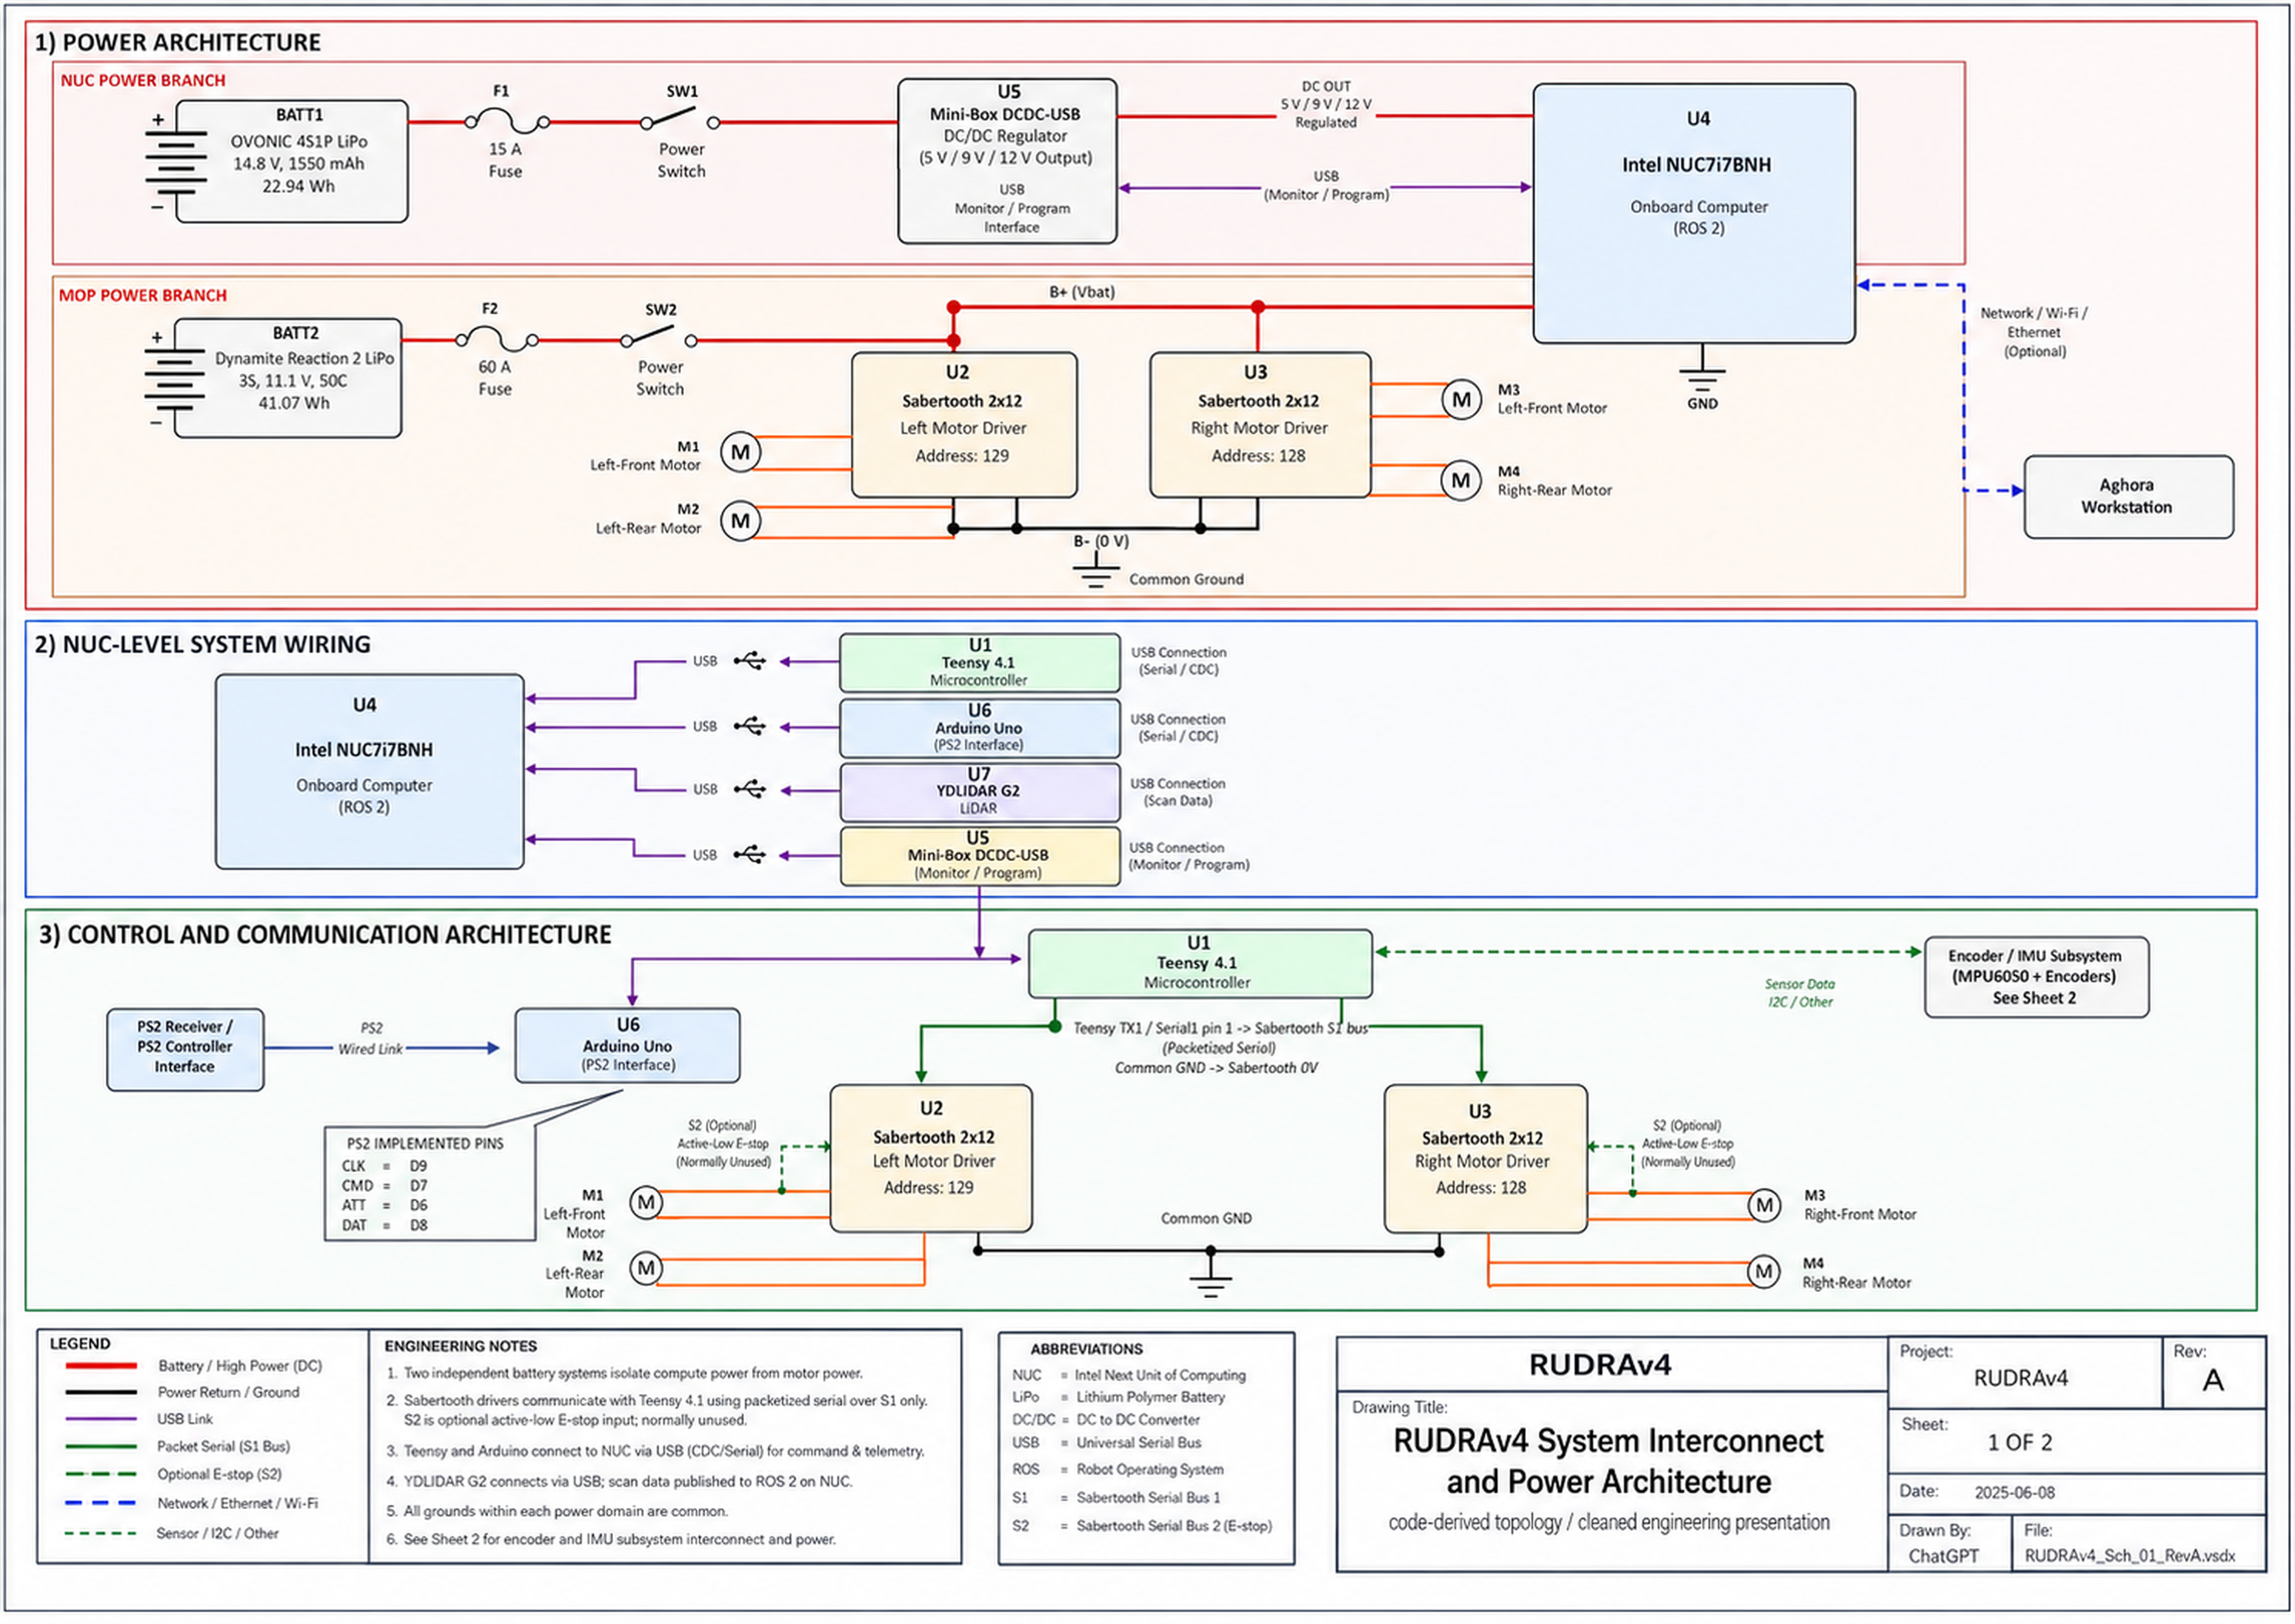
\includegraphics[width=0.96\linewidth,height=0.82\textheight,keepaspectratio]{figures/schematics/rudrav4_system_interconnect_schematic_highres.png}
\caption{RUDRAv4 Sheet 1 of 2: system interconnect and power architecture.  This sheet shows the NUC power branch through the Mini-Box DCDC-USB, the motor power branch through the Sabertooth drivers, the NUC USB wiring to Teensy/Uno/YDLIDAR/DCDC-USB, and the high-level control and communication architecture.}
\label{fig:rudra-sch-sheet1}
\end{figure}
\end{landscape}

\begin{landscape}
\begin{figure}[p]
\centering
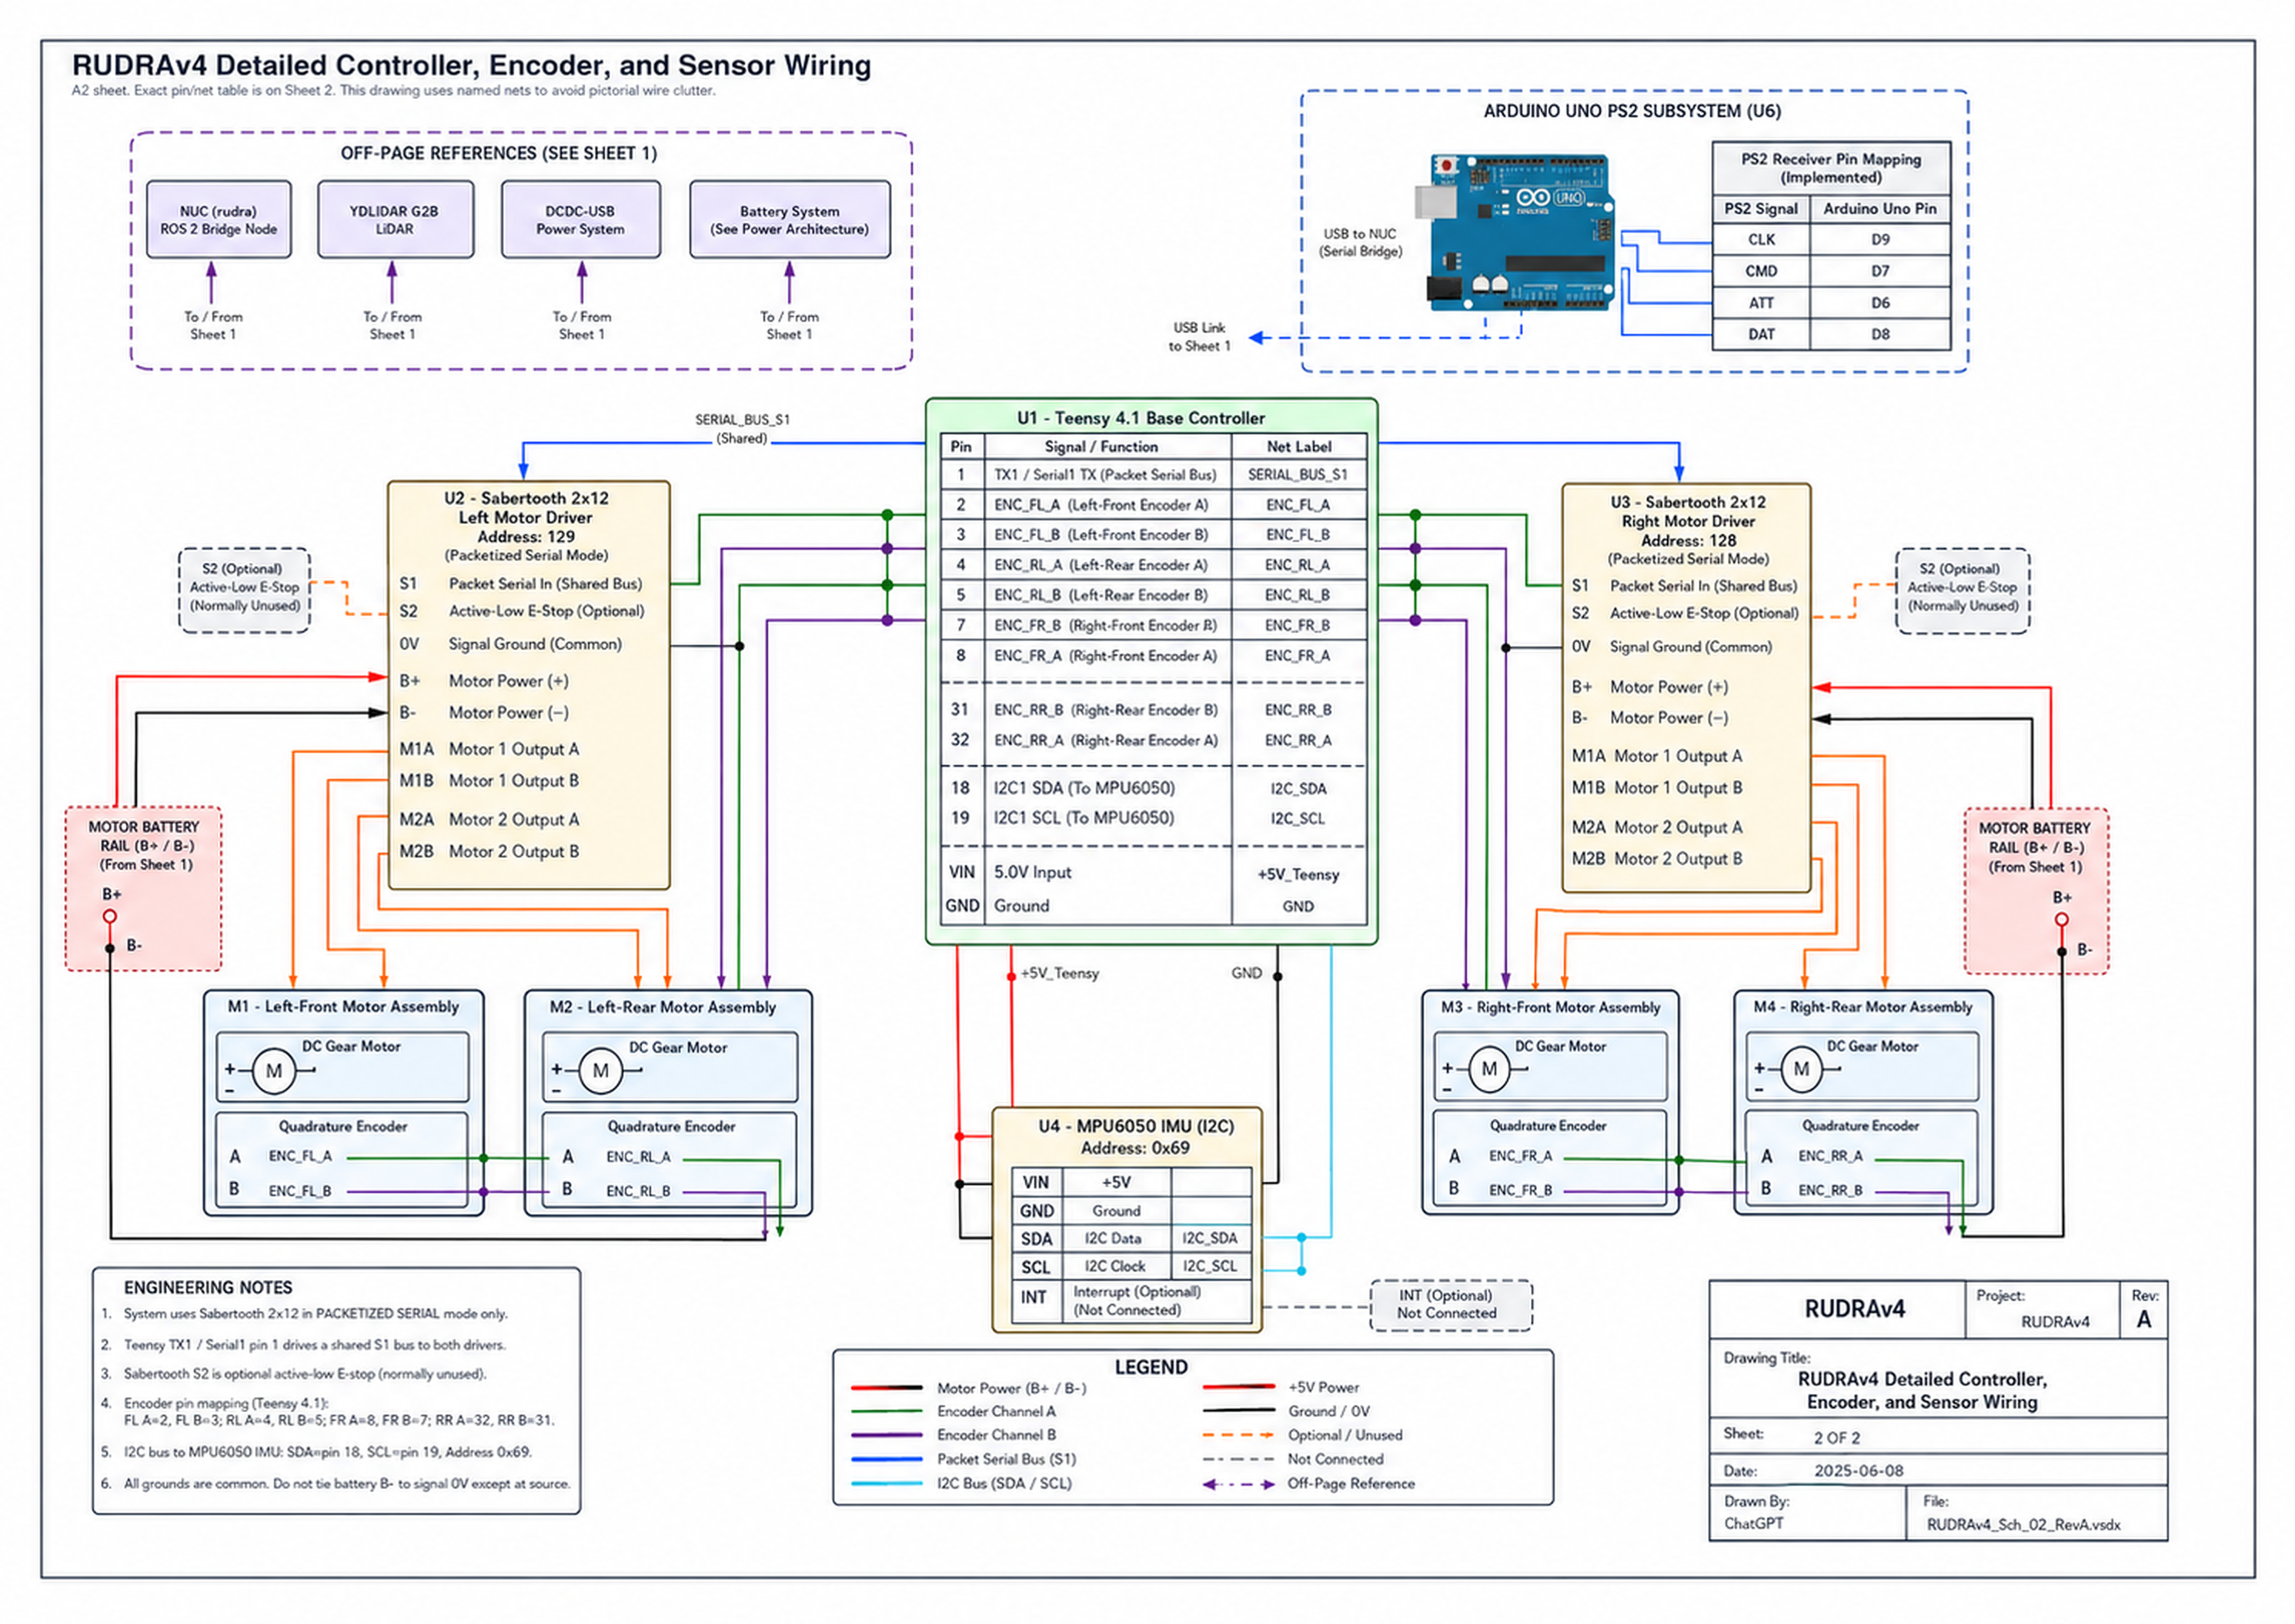
\includegraphics[width=0.96\linewidth,height=0.82\textheight,keepaspectratio]{figures/schematics/rudrav4_controller_wiring_schematic_highres.png}
\caption{RUDRAv4 Sheet 2 of 2: detailed controller, encoder, and sensor wiring.  This sheet documents the implemented Teensy pin mapping, shared packetized-serial Sabertooth S1 bus, optional S2 e-stop concept, motor/encoder wiring, MPU6050 I2C wiring, and Arduino Uno PS2 receiver pin mapping.}
\label{fig:rudra-sch-sheet2}
\end{figure}
\end{landscape}

\section{Schematic interpretation notes}

The two-sheet schematic set should be read with the firmware contracts in \cref{chap:teensy-uno-ps2,chap:sabertooth}.  The important implementation constraints are:

\begin{itemize}
  \item Sabertooth command is packetized serial, not PWM/DIR.
  \item Teensy \cmd{TX1}/\cmd{Serial1} drives the shared Sabertooth \cmd{S1} bus.
  \item Sabertooth \cmd{S2} is shown as optional active-low emergency stop and is not used as an RX channel.
  \item The NUC owns the ROS graph and connects by USB to the Teensy, Uno, YDLIDAR, and DCDC-USB monitor/programming interface.
  \item The NUC LiPo and motor LiPo are separate power branches; grounds are handled intentionally at the documented boundaries.
\end{itemize}
